\section{Results}
\label{Results}

\subsection{Baseline \& Feature Selection results}
The baseline characteristics for the included patients are shown in Table \ref{tab:descriptives}. A total of 76 patients with 713 independent periods have been included. The prevalence of NH for these periods was 15.8 \% for the included patients. The average age was at 64.9 years (SD= 9.8) and the majority of patients were male (62.3 \%). The study population had a high average BMI of 30.5 (SD= 4.9).

Boruta feature selection and MI criteria identified the most important variables for the two data conditions. The Boruta approach revealed that in the full data condition, only two features (AOB and Diabetes duration) were included that were not extracted from CGM values. Further, CGM indices and descriptive statistics for the intervals of zero to one hour and over six hours before bedtime were considered the most important features. In the Lifestyle condition, features from all categories except temporal location were selected. The most important features were baseline patient characteristics, including BMI, height, and weight, followed by features from both lifestyle categories. The ten most important features based on Boruta for both conditions are shown in Figure \ref{fig:features}.
The results of the MI criteria mostly supported the decisions based on Boruta. Additionally, MI criteria identified several baseline characteristics (BMI, HbA1c values, weight, height, and age) that clearly shared information with the outcome variable. Within the lifestyle features, MI indicated that AOB, the sum of steps, and ingested calories shared most information with the outcome variable. Both feature selection methods suggested that medication- and temporal-location features were the least important for this predictive task.

\subsection{Model comparison}
In this study, the performance of 80 independent models using various ML algorithms, sampling and tuning strategies, and data conditions were evaluated. Specifically, four ML algorithms (RF, SVM, XGB, and Lasso) with three sampling strategies (Original, Smote, and Up-sampling), three tuning strategies (Default Grid, Random Grid, and Customized Grid), and two data conditions (Full data condition \& Lifestyle condition) were tested, resulting in a total of (4*3*3*2) 72 models. All of these models applied cost-sensitive learning by threshold moving. Additionally, for each combination of an ML algorithm and data condition (4*2), models with a threshold set to .5 for the prediction of the outcome, resulting in 8 additional models. This approach was repeated three times using different training and test data divisions, where means and SDs were conducted for each of the 80 models.

The best-performing tuning strategy, based on the model's average performance on the evaluation metrics, for each combination of an ML algorithm and sampling approach was selected, which resulted in a total of 32 models, presented in Table \ref{tab:results_all}. Across the selected models no superior tuning strategy could be identified.

The results showed that using sampling strategies to address the class imbalance, such as SMOTE and Up-Sampling, did not lead to better results compared to using the original data sampling. For the full data condition, the original sampling resulted in the best performance across all ML algorithms (AUC=0.88-0.91, SENS=0.85-0.89, SPEC=0.78-0.87). For the Lifestyle condition, no superior sampling strategy was identified for all evaluation metrics, but Up-Sampling showed less variability in its estimates compared to the original sampling. Although the difference between the three sampling methods was small in terms of AUC, it fluctuated more for both SENS and SPEC.

The findings further revealed that the cost-sensitive learning approach consistently resulted in higher SENS across all ML algorithms when compared to the models trained without cost-sensitive learning. Specifically, in the Lifestyle condition,  the difference in SENS is highest between the models that applied threshold moving compared to the no-cost models (SENS No-Cost=0.06-0.31, SENS Original=0.78-0.83).

Last, the results demonstrated that the choice of ML algorithm had only a minor impact on the evaluation metrics in the Full data condition, with RF (AUC=0.88-0.91, SENS=0.88-0.89, SPEC=0.75-0.83) achieving the best results, followed by XGB, SVM, and Lasso. In contrast, in the Lifestyle condition, while RF still performed the best, with XGB and SVM following closely, Lasso performed significantly worse in terms of AUC and SPEC. Specifically, Lasso achieved a much lower AUC (0.58) and lower SPEC (0.41-0.49) compared to other algorithms, although its SENS was still relatively high (0.73-0.80).

\newcommand*{\MyIndent}{\hspace*{0.5cm}}
\begin{table}[tb]
  \sf\centering
  \caption{Baseline Characteristics of Patients \textit{N = 76}.}
  \begin{tabular}{lcc}
    \hline
    \textbf{Variable} & \textbf{Mean (Proportion)}  & \textbf{SD (\%)} \\
    \hline
    
    Nocturnal Hypo. \\
       \MyIndent Yes & 113 & 15.8 \% \\   
       \vspace{0.15cm}
      \MyIndent No    & 600 & 84.2 \% \\
      \vspace{0.15cm}
    Age (years)& 64.9 & $\pm$ 9.8 \\
    Gender \\
       \MyIndent Female & 269 & 37.7 \% \\   
       \vspace{0.15cm}
      \MyIndent Male    & 444 & 62.3 \% \\
      \vspace{0.15cm}
    Height (cm) & 173.3 & $\pm$ 9.2 \\
    \vspace{0.15cm}
    Weight (kg) & 91.4 & $\pm$ 14.8 \\
    \vspace{0.15cm}
    BMI (kg/m^2) & 30.5 & $\pm$ 4.9 \\
    \vspace{0.15cm}
    HbA1c (mmol/mol) & 56.7 & $\pm$ 11.9 \\ 
    \vspace{0.15cm}
    Duration T2D (years) & 17.7 & $\pm$ 9.9 \\
    \hline
    \end{tabular} %
      \label{tab:descriptives}%
    \vspace{0.25cm}
  \parbox{0.45\textwidth}{\small{\textit{Note:} Continuous variables are presented by mean ± standard deviation and categorical variables by percentage (proportion).}}
\end{table}
  
\begin{table*} [tb]
\sf\centering
\caption{Averaged Performance Metrics and Standard Deviations for Model Comparison.}
\label{table:performance_metrics}
\begin{tabular}{cc|cccc|cccc}
\hline
\multicolumn{2}{c}{\textbf{}} & \multicolumn{4}{c}{\textbf{Full Data Condition}} & \multicolumn{4}{c}{\textbf{Lifestyle Condition}} \\ \cline{3-10} 
\textbf{Model} & \textbf{Metric} & \textbf{No-Cost} & \textbf{Original} & \textbf{SMOTE} & \textbf{Up} &  \textbf{No-Cost} & \textbf{Original} & \textbf{SMOTE} & \textbf{Up} \\ \hline
\multirow{\textbf{RF}} & \textbf{AUC}& 0.90 & \textbf{0.91} & 0.88 & 0.88 & 0.81 & 0.82 & 0.82 & 0.81 \\ 
& & (0.04) & \textbf{(0.03)} & (0.01) & (0.01) & (0.04) & (0.03) & (0.02) & (0.04) \\ 
 & \textbf{SENS} & 0.33 & \textbf{0.89} & 0.88 & 0.88 & 0.21 & 0.83 & 0.81 & 0.80 \\  
 & & (0.20) & \textbf{(0.08)} & (0.06) & (0.04) & (0.05) & (0.05) & (0.07) & (0.08) \\
 & \textbf{SPEC} & 0.97 & 0.83 & 0.78 & 0.75 & 0.97 & 0.69 & 0.71 & 0.72 \\ 
& & (0.03) & (0.05) & (0.05) & (0.01) & (0.02) & (0.07) & (0.06) & (0.04) \\  \hline
\multirow{\textbf{SVM}} & \textbf{AUC} & 0.89 & 0.89 & 0.86 & 0.88 & 0.78 & 0.78 & 0.78 & 0.78 \\  
& & (0.04) & (0.04) & (0.04) & (0.02) & (0.05) & (0.05) & (0.05) & (0.04) \\
 & \textbf{SENS} & 0.35 & 0.86 & 0.89 & 0.82 & 0.06 & 0.82 & 0.80 & 0.79 \\
& & (0.13) & (0.02) & (0.06) & (0.04) & (0.02) & (0.07) & (0.08) & (0.03) \\ 
 & \textbf{SPEC} & 0.97 & 0.87 & 0.70 & 0.84 & \textbf{1.00} & 0.60 & 0.67 & 0.66 \\   
& & (0.02) & (0.08) & (0.04) &( 0.02) & \textbf{(0.00)} & (0.05) & (0.10) & (0.07) \\  \hline
\multirow{\textbf{XGB}} & \textbf{AUC} & 0.89 & 0.90 & 0.89 & 0.90 & 0.81 & 0.81 & 0.79 & 0.78 \\  
& & (0.04) & (0.06) & (0.04) & (0.04) & (0.03) & (0.03) & (0.04) & (0.04) \\ 
 & \textbf{SENS} & 0.52 & 0.86 & \textbf{0.89} & 0.87 & 0.31 & 0.79 & 0.84 & 0.82 \\ 
& & (0.10) & (0.06) & \textbf{(0.03)} & (0.09) & (0.04) & (0.04) & (0.03) & (0.04) \\ 
 & \textbf{SPEC} & 0.95 & 0.82 & 0.78 & 0.81 & 0.97 & 0.74 & 0.62 & 0.64 \\ 
& & (0.03) & (0.06) & (0.07) & (0.06) & (0.00) & (0.04) & (0.03) & (0.05) \\ \hline
\multirow{\textbf{Lasso}} & \textbf{AUC}  & 0.88 & 0.88 & 0.85 & 0.86 & 0.58 & 0.58 & 0.58 & 0.58 \\ 
& & (0.06) & (0.05) & (0.07) & (0.05) & (0.05) & (0.06) & (0.03) & (0.06) \\ 
 & \textbf{SENS} & 0.38 & 0.85 & 0.83 & 0.82 & 0.22 & 0.78 & 0.80 & 0.73 \\  
& & (0.04) & (0.04) & (0.05) & (0.06) & (0.30) & (0.08) & (0.12) & (0.04) \\
 & \textbf{SPEC} & 0.96 & 0.78 & 0.74 & 0.76 & 0.81 & 0.45 & 0.41 & 0.49 \\ 
& & (0.01) & (0.06) & (0.14) & (0.05) & (0.17) & (0.03) & (0.10) & (0.04) \\ \hline
\end{tabular} %
\label{tab:results_all}%
 \vspace{0.25cm}
  \parbox{0.8\textwidth}{\small{\textit{Note:} The results are averaged over three folds and SDs are depicted within parentheses. Models are shown for 4 ML algorithms, with 3 distinct sampling strategies, and 2 data conditions. Models excluding cost-sensitive learning are shown in the columns "No Cost".  }}
\end{table*}%

\subsection{Difference between Lifestyle and CGM data}
This second part of the analysis focused on the comparison of the two data conditions. Only models using cost-sensitive learning were considered for comparison.

The results suggested that the inclusion of CGM features consistently resulted in higher AUC values compared to subsets without CGM, with AUC ranging from 0.85 to 0.91 for the Full data condition and 0.58 to 0.82 for the Lifestyle condition. In terms of SENS, the Full data condition ranged between 0.82 to 0.89, while the Lifestyle condition led to similar estimates, with SENS ranging from 0.73 to 0.84. In terms of SPEC, there was a consistently lower performance in the Lifestyle condition, with SPEC ranging from 0.41 to 0.74, compared to 0.70 to 0.87 for the Full data condition. The results of the ROC analysis for the two data conditions across the four ML algorithms and over the three folds are depicted in Figure \ref{fig:roc_curves}.

\begin{figure}[htbp]
\sf\centering
\caption{ROC curve comparison - Full Data Condition vs. Lifestyle Condition across all ML algorithms.}
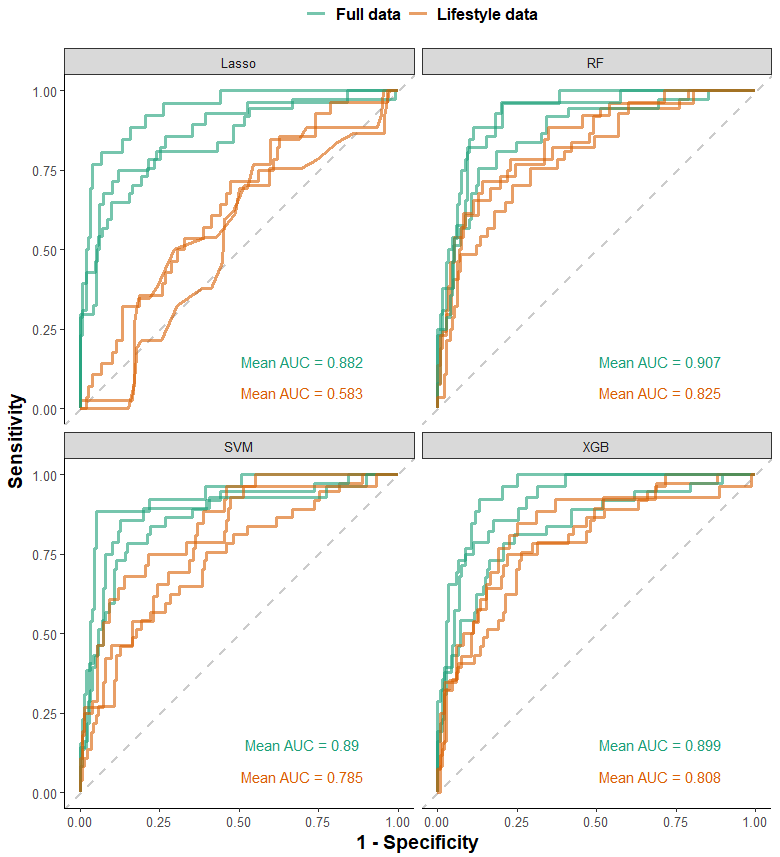
\includegraphics[width=0.5\textwidth]{Figures/ROC_compare_folds_rs.png}
\vspace{0.25cm}
  \parbox{0.45\textwidth}{\small{\textit{Note:} Same model building choices were applied across all three folds .}}
\label{fig:roc_curves}
\end{figure}